\documentclass[11pt,letterpaper]{article}
\usepackage[lmargin=1in,rmargin=1in,tmargin=1in,bmargin=1in]{geometry}
\usepackage{../style/homework}
\usepackage{../style/commands}
\setbool{quotetype}{false} % True: Side; False: Under
\setbool{hideans}{true} % Student: True; Instructor: False

% -------------------
% Content
% -------------------
\begin{document}

\homework{3: Due 09/??}{}{}

% Problem 1
\problem{10} Two relations, $F$ and $G$, are represented below. Are either $F$ or $G$ functions? Explain. 
	\[
	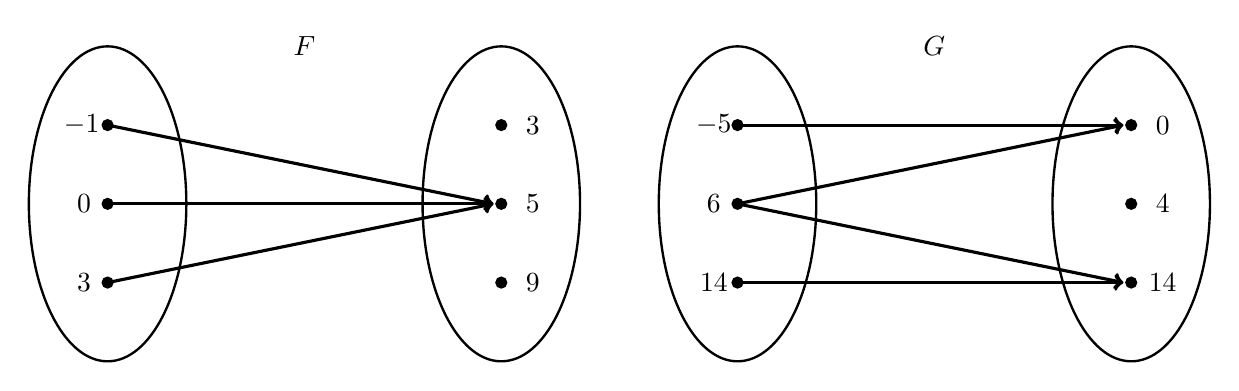
\begin{tikzpicture}
	\node at (2.5,2) {$F$};
	% Ellipses
	\draw[line width=0.03cm] (0,0) circle (1 and 2);
	\draw[line width=0.03cm] (5,0) circle (1 and 2);
	
	% Nodes
	\draw[fill=black] (0,1) circle (0.07);
	\draw[fill=black] (0,0) circle (0.07);
	\draw[fill=black] (0,-1) circle (0.07);
	
	\draw[fill=black] (5,1) circle (0.07);
	\draw[fill=black] (5,0) circle (0.07);
	\draw[fill=black] (5,-1) circle (0.07);
	
	% Arrow
	\draw[line width=0.04cm,->] (0,1) -- (4.9,0);
	\draw[line width=0.04cm,->] (0,0) -- (4.9,0);
	\draw[line width=0.04cm,->] (0,-1) -- (4.9,0);
	
	% Labels
	\node at (-0.3,1) {$-1$\,};
	\node at (-0.3,0) {$0$};
	\node at (-0.3,-1) {$3$};
	
	\node at (5.4,1) {$3$};
	\node at (5.4,0) {$5$};
	\node at (5.4,-1) {$9$};
	
	\tikzset{shift={(8,0)}}
	%
	\node at (2.5,2) {$G$};
	% Ellipses
	\draw[line width=0.03cm] (0,0) circle (1 and 2);
	\draw[line width=0.03cm] (5,0) circle (1 and 2);
	
	% Nodes
	\draw[fill=black] (0,1) circle (0.07);
	\draw[fill=black] (0,0) circle (0.07);
	\draw[fill=black] (0,-1) circle (0.07);
	
	\draw[fill=black] (5,1) circle (0.07);
	\draw[fill=black] (5,0) circle (0.07);
	\draw[fill=black] (5,-1) circle (0.07);
	
	% Arrow
	\draw[line width=0.04cm,->] (0,1) -- (4.9,1);
	\draw[line width=0.04cm,->] (0,0) -- (4.9,1);
	\draw[line width=0.04cm,->] (0,0) -- (4.9,-1);
	\draw[line width=0.04cm,->] (0,-1) -- (4.9,-1);
	
	% Labels
	\node at (-0.3,1) {$-5$};
	\node at (-0.3,0) {$6$};
	\node at (-0.3,-1) {$14$};
	
	\node at (5.4,1) {$0$};
	\node at (5.4,0) {$4$};
	\node at (5.4,-1) {$14$};
	\end{tikzpicture}
	\]



\newpage



% Problem 2
\problem{10} Given the following tables, do $f(x)$ and $g(x)$ represent functions? Explain. 
	\begin{table}[!ht]
	\centering \setlength\arrayrulewidth{0.02cm}
	\begin{tabular}{c|ccc|c} 
	$x$ & $f(x)$ & \hspace{2cm} & $x$ & $g(x)$ \\ \cline{1-2} \cline{4-5}
	$1$ & $1$ && $1$ & $0$ \\
	$2$ & $3$ && $2$ & $3$ \\
	$3$ & $5$ && $3$ & $3$ \\
	$4$ & $0$ && $4$ & $6$ \\
	$5$ & $3$ && $1$ & $7$  
	\end{tabular}
	\end{table}
	


\newpage



% Problem 3
\problem{10} Does the formula $f(x):= 1.67x + 5.34$ give a function? 




\vfill 












%\printpoints
\end{document}